\chapter{Konzept}
\label{cha:konzept}
Der Aufbau und das Systemdesign des Aktivitäts-Tracking-Frameworks bilden einen zentralen Bestandteil dieser Arbeit. In diesem Kapitel werden die einzelnen Komponenten beschrieben, die für das Tracking von Aktivitätsdaten erforderlich sind. Die praktische Umsetzung des Konzepts erfolgt anschließend in Kapitel \ref{cha:implementierung}.

\section{Systemarchitektur}
Bevor die einzelnen Komponenten im Detail erläutert werden, beschreibt dieser Abschnitt die Zusammenarbeit und die übergeordnete Struktur der Teilbereiche und Systemkomponenten.

\subsection{Komponenten und Aufbau}
\label{sec:system_design}
Das Tracking-Framework besteht aus sechs Teilbereichen, die gemeinsam den gesamten Funktionsumfang des Systems abdecken:

\begin{itemize}
    \item Systemkonfiguration
    \item Trackingkonfiguration
    \item Daten- und Aktionsermittlung
    \item Filterung und Extraktion
    \item Vermittlung und Ablaufsteuerung
    \item Datenaustausch und Zwischenspeicherung
\end{itemize}

Im Rahmen der Implementierung (siehe Kapitel \ref{cha:implementierung}) wurden diese Teilbereiche in eigenständige Komponenten unterteilt. Abbildung~\ref{fig:system_design_components} zeigt, wie diese Komponenten im System zusammenarbeiten.

Das zentrale Element bildet der Tracking-Manager, über den alle Komponenten miteinander verbunden sind. Jede Komponente verfügt über eine klar definierte Schnittstelle, die den Zugriff ermöglicht. Nur der Tracking-Manager kennt die einzelnen Komponenten, während diese untereinander vollständig entkoppelt und unabhängig agieren.

Diese Struktur sorgt für eine hohe Flexibilität. Änderungen, die von der Systemumgebung abhängen, können vorgenommen werden, ohne andere Teile des Frameworks zu beeinflussen. So lässt sich beispielsweise die Art der Datenverarbeitung anpassen, ohne dass der übrige Aufbau geändert werden muss.

\begin{figure}[H]
    \centering
    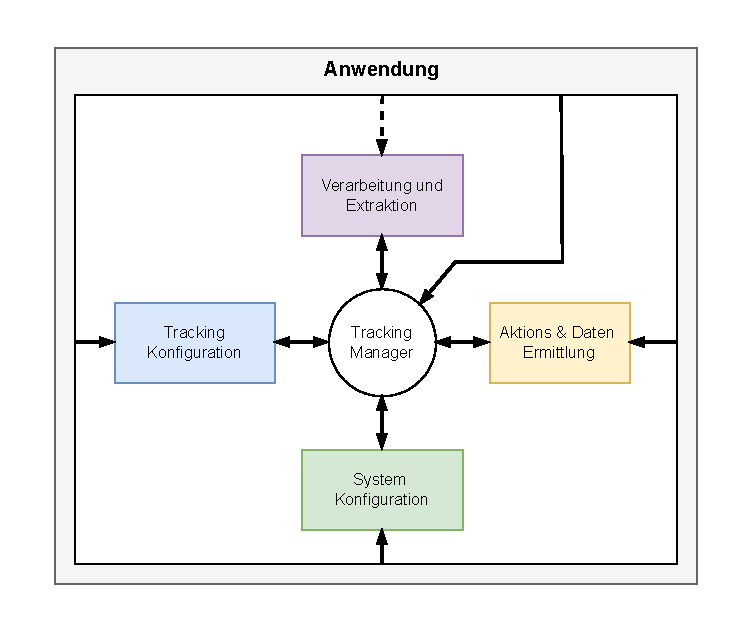
\includegraphics[width=0.8\textwidth]{5_Systemdesign_Components_Tracking}
    \caption{Zusammenhänge der Komponenten im Tracking-Framework}
    \label{fig:system_design_components}
\end{figure}

Die lose Kopplung besteht nicht nur zwischen den internen Komponenten des Frameworks, sondern auch zwischen der Anwendung und der Datensammlung (siehe Abbildung \ref{fig:system_design_components}). Welche Daten erfasst werden und an welcher Stelle die Erhebung erfolgt, wird vollständig durch das Framework gesteuert. 

Die Anwendung selbst muss im Wesentlichen lediglich die erforderlichen Daten über eine definierte Schnittstelle bereitstellen. Dadurch lässt sich das System flexibel in unterschiedlichen Technologien einsetzen, beispielsweise in WPF (siehe Unterabschnitt~\ref{subsec:WPF}) oder Windows Forms (siehe Unterabschnitt~\ref{subsec:Winforms}).

\section{Tracking Konfiguration}
\label{sec:configuration_concept}

\section{Daten- und Aktionsermittlung}
\label{sec:data_collection_concept}

\section{Filterung und Extraktion}
\label{sec:data_extraction_concept}

\section{Einbettung in bestehende Systeme}
\label{sec:integration_concept}


